\documentclass[11pt,a4paper]{article}

\usepackage[utf8]{inputenc}
\usepackage{lmodern}
\usepackage[T1]{fontenc}
\IfFileExists{french.ldf}{\usepackage[french]{babel}}{}
\renewcommand{\contentsname}{Table des matières}
\renewcommand{\figurename}{Figure}
\renewcommand{\tablename}{Tableau}
\renewcommand{\refname}{Références}
\usepackage{geometry}
\usepackage{graphicx}
\usepackage{xcolor}
\usepackage{amsmath,amssymb}
\usepackage{booktabs}
\usepackage{tabularx}
\usepackage{array}
\usepackage{float}
\usepackage{caption}
\usepackage{enumitem}
\usepackage{fancyhdr}
\usepackage{listings}
\usepackage{titlesec}
\usepackage{indentfirst}
\usepackage{hyperref}

\geometry{margin=2.4cm,headheight=15pt}
\definecolor{titreNoir}{HTML}{000000}
\definecolor{fondCommandes}{HTML}{FAF5EF}
\definecolor{bordCommandes}{HTML}{79523A}
\hypersetup{
  colorlinks=true,
  linkcolor=titreNoir,
  urlcolor=titreNoir,
  citecolor=titreNoir,
  pdftitle={Explications - Projet Analyse de la structure des membranes lipidiques},
  pdfauthor={BERNARD Valentin, BRAHAM Amyne, FOURNAISE Antoine, ZAMOUM Tassadit},
}
\setlength{\parindent}{1.4em}
\setlength{\parskip}{0pt}
\linespread{1.08}
\raggedbottom
\setlist[itemize]{leftmargin=*,topsep=2pt,itemsep=2pt}
\setlist[enumerate]{leftmargin=*,topsep=2pt,itemsep=2pt}
\renewcommand{\arraystretch}{1.25}
\titleformat{\section}{\Large\bfseries}{\thesection\ --}{0.5em}{}
\titleformat{\subsection}{\large\bfseries}{\thesubsection\ --}{0.5em}{}
\titleformat{\subsubsection}{\normalsize\bfseries}{\thesubsubsection\ --}{0.5em}{}
\titleformat{\paragraph}[block]{\normalsize\bfseries}{}{0pt}{}
\titlespacing*{\section}{0pt}{1.6em}{0.9em}
\titlespacing*{\subsection}{0pt}{1.3em}{0.6em}
\titlespacing*{\paragraph}{0pt}{1.1em}{0.4em}
\captionsetup{font=small,labelfont=bf,justification=centering,width=0.9\textwidth,skip=6pt}
\captionsetup[table]{font=small,labelfont=bf,justification=raggedright,singlelinecheck=false,width=\textwidth,skip=5pt,position=top}
\captionsetup[lstlisting]{font=small,labelfont=bf,justification=centering,skip=6pt}
\lstdefinestyle{terminal}{
  basicstyle=\ttfamily\small,
  backgroundcolor=\color{fondCommandes},
  frame=single,
  rulecolor=\color{bordCommandes},
  breaklines=true,
  columns=fullflexible,
  keepspaces=true,
  showstringspaces=false,
  xleftmargin=0.3em,
  xrightmargin=0.3em,
  extendedchars=true,
  aboveskip=1.1em,
  belowskip=1.1em,
  literate={é}{{\'e}}1 {è}{{\`e}}1 {ê}{{\^e}}1 {à}{{\`a}}1 {ç}{{\c{c}}}1
           {É}{{\'E}}1 {ô}{{\^o}}1 {î}{{\^i}}1 {ù}{{\`u}}1 {œ}{{\oe}}1 {û}{{\^u}}1 {µ}{{$\mu$}}1
}
\lstset{style=terminal}
\makeatletter\newcommand{\tabinput}[1]{\@@input #1 }\makeatother

% membres du groupe, par ordre alphabetique du nom de famille
\newcommand{\auteurUn}{\textsc{Bernard} Valentin}
\newcommand{\auteurDeux}{\textsc{Braham} Amyne}
\newcommand{\auteurTrois}{\textsc{Fournaise} Antoine}
\newcommand{\auteurQuatre}{\textsc{Zamoum} Tassadit}
\newcommand{\enseignant}{\textsc{Crowet} Jean-Marc}
\newcommand{\formation}{Master 2 Calcul Haute Performance et Simulation (CHPS)}
\newcommand{\anneeUniv}{2026--2027}
\newcommand{\dateRapport}{25 novembre 2026}

\pagestyle{fancy}
\fancyhf{}
\fancyhead[L]{\small Éléments de bioinformatique : le HPC en biologie}
\fancyhead[R]{\small Explications -- Projet membranes lipidiques}
\fancyfoot[C]{\thepage}
\renewcommand{\headrulewidth}{0pt}
\renewcommand{\footrulewidth}{0pt}

\definecolor{boxbg}{HTML}{EEF4FB}
\definecolor{boxrule}{HTML}{2A78D6}
\newcommand{\fichiers}[1]{%
  \par\smallskip\noindent\fcolorbox{boxrule}{boxbg}{\parbox{\dimexpr\linewidth-2\fboxsep-2\fboxrule}{%
  \small\sloppy\setlength{\parindent}{0pt}\textbf{Fichiers correspondants}\par\vspace{0.2em}#1}}\par\smallskip}
\newcommand{\f}[1]{\texttt{#1}}

\begin{document}
\hypersetup{pageanchor=false}
\begin{titlepage}
\thispagestyle{empty}
\centering
\vspace*{0.65cm}

\includegraphics[width=0.46\textwidth,keepaspectratio]{figures/logo-urca-officiel.png}\\[1.05cm]
{\Large Université de Reims Champagne-Ardenne\par}
\vspace{0.35cm}
{\large \formation\par}
\vspace{0.35cm}
{\normalsize UE Éléments de bioinformatique : utilisation du HPC dans la biologie (CHPS1001)\par}
\vspace{1.45cm}
{\Huge\bfseries\color{titreNoir} Explications détaillées\par}
\vspace{0.35cm}
{\LARGE Projet : analyse de la structure\\[0.15cm]
des membranes lipidiques\par}
\vspace{0.3cm}
{\large Ce qui a été fait, pourquoi, et où le trouver\par}
\vspace{1.5cm}
{\normalsize\bfseries Membres du groupe\par}
\vspace{0.3cm}
{\large
\auteurUn\par\vspace{0.12cm}
\auteurDeux\par\vspace{0.12cm}
\auteurTrois\par\vspace{0.12cm}
\auteurQuatre\par}
\vspace{0.9cm}
{\normalsize\bfseries Enseignant\par}
\vspace{0.3cm}
{\large \enseignant\par}
\vfill
{\large Année universitaire \anneeUniv\par}
{\normalsize \dateRapport\par}
\end{titlepage}
\hypersetup{pageanchor=true}
\sloppy
\setcounter{page}{1}
\begingroup
\setcounter{tocdepth}{2}
\tableofcontents
\endgroup
\clearpage

\noindent\textit{Ce document explique le projet point par point. Ce n'est pas le rapport à rendre~: le rapport
est \f{doc\_Projet/rapport/rapport.pdf}. Ici, on explique simplement chaque étape et on indique, à chaque fois, les fichiers
du dossier qui y correspondent.}

%=====================================================================
\section{Comprendre le sujet}
%=====================================================================
\subsection{Qu'est-ce qu'un feuillet~?}
Une membrane biologique est formée de deux couches de lipides, appelées \textbf{feuillets}. Un lipide est
\emph{amphiphile}~: il possède une \textbf{tête} qui aime l'eau (hydrophile) et une \textbf{queue} qui la fuit
(hydrophobe). Dans chaque feuillet, les têtes sont tournées vers l'eau et les queues vers le milieu de la
membrane~: les deux feuillets sont donc placés « dos à dos ».

Dans une \textbf{bicouche plane}, il y a un feuillet du haut et un feuillet du bas. Dans une
\textbf{vésicule} (une petite bulle de membrane), il y a un feuillet extérieur et un feuillet intérieur.

\subsection{Que demande le projet~?}
Écrire un programme qui dit, pour chaque lipide, \textbf{à quel feuillet il appartient}, de façon
\textbf{fiable} et \textbf{rapide}. La rapidité compte parce qu'une simulation produit une
\emph{trajectoire} de dizaines de milliers d'images, et qu'il faut refaire l'analyse sur chacune~: des lipides
peuvent changer de feuillet au cours du temps (phénomène de \emph{flip-flop}).

L'énoncé demande six choses~:
\begin{enumerate}
\item une version utilisant un \textbf{graphe} avec une \textbf{recherche automatique du seuil}~;
\item une version qui n'a \textbf{pas besoin qu'on lui dise quel atome est la tête} de chaque lipide~;
\item une version utilisant l'\textbf{orientation} des lipides et la \textbf{normale locale} à la membrane~;
\item une \textbf{version finale} qui ne garde que l'essentiel, avec une justification~;
\item l'application de la version finale à une \textbf{trajectoire}, avec mesure du temps~;
\item une \textbf{comparaison} avec deux outils existants, \textbf{LeafletFinder} et \textbf{FATSLiM}.
\end{enumerate}

\subsection{Les données fournies}
Le dossier \f{Projet3/} contient 7 membranes. Pour chacune, il y a deux fichiers~:
\begin{itemize}
\item un fichier \f{.gro}~: la position de chaque atome à un instant donné (une « photo » de la membrane)~;
\item un fichier \f{leaflets.txt}~: la bonne réponse, c'est-à-dire la liste des lipides de chaque feuillet.
Elle sert à mesurer si notre programme a raison.
\end{itemize}

\begin{table}[H]\centering\small
\begin{tabular}{|l|r|l|}\hline
Membrane & Lipides & Description\\\hline
\f{bilayer\_chol} & 1944 & bicouche plane avec cholestérol (gros grains)\\\hline
\f{bilayer\_peptide} & 126 & petite bicouche avec un peptide (united-atom)\\\hline
\f{bilayer\_prot} & 112 & petite bicouche avec 5 peptides (united-atom)\\\hline
\f{model\_vesicle} & 2748 & vésicule idéale construite par ordinateur (united-atom)\\\hline
\f{dppc\_vesicle} & 3072 & vésicule formée spontanément en simulation (gros grains)\\\hline
\f{small\_plasma\_membrane} & 6664 & membrane plasmique réaliste, 65 types de lipides\\\hline
\f{large\_plasma\_membrane} & 19\,239 & grande membrane plasmique, 63 types de lipides\\\hline
\end{tabular}
\caption{Les 7 membranes fournies. « Gros grains » (CG)~: plusieurs atomes sont regroupés en une seule bille~;
« united-atom » (UA)~: les hydrogènes des groupes méthyle ne sont pas représentés.}
\end{table}

\textbf{La trajectoire.} Un fichier \f{.gro} ne contient qu'une seule image. Une \emph{trajectoire} est un
« film »~: une suite d'images, dans un fichier \f{.xtc} ou \f{.trr}. La trajectoire du cours est dans le dossier
\f{Surfactine-R1/}~: c'est une simulation GROMACS (modèle Martini~3) d'une membrane plane de 3040 lipides (PIPC,
glucosylcéramide GCER et cholestérol) avec 96 molécules de \textbf{surfactine}, un lipopeptide bactérien. Les
fichiers utiles sont~:
\begin{itemize}
\item \f{prod.gro}~: la structure (positions et noms des 83\,095 particules)~;
\item \f{prod.tpr}~: la topologie GROMACS, qui dit quels atomes forment chaque molécule~;
\item \f{prod\_dt1000ns.xtc}~: la simulation de production, 20\,µs, une image par µs (21 images)~;
\item \f{prod1.xtc}~: la phase où les surfactines sont tirées vers la membrane, 5\,ns, 1001 images~;
\item \f{prod.trr}~: la production, mais le fichier est \textbf{incomplet} (61 images lisibles)~;
\item \f{prod\_pep.xtc}~: uniquement les peptides, sans lipides~: inutilisable pour les feuillets.
\end{itemize}
Avant d'avoir cette trajectoire, le programme avait été mis au point sur une petite trajectoire de la vésicule DPPC
(11 images, fournie avec FATSLiM), rangée dans \f{trajectoire/}.

\fichiers{%
\f{2026\_CHPS1001\_Projet\_Analyse\_de\_Membranes\_Lipidiques.pdf}~: l'énoncé.\\
\f{Projet3/<membrane>/<membrane>.gro}~: les 7 structures.\\
\f{Projet3/<membrane>/leaflets.txt}~: les bonnes réponses.\\
\f{Projet3.zip}~: l'archive d'origine (même contenu que \f{Projet3/}).\\
\f{Surfactine-R1/}~: la trajectoire du cours.\\
\f{trajectoire/dppc\_vesicle.gro} et \f{.xtc}~: la trajectoire de test utilisée au début.}

%=====================================================================
\section{L'installation des logiciels}
%=====================================================================
Ce qui était déjà sur le PC~: le compilateur C++ \f{gcc} (avec OpenMP pour le calcul parallèle), Python~3.14,
NumPy, VMD (visualisation de molécules) et \LaTeX{} (pour produire les PDF).

Ce qui a été installé, sans mot de passe administrateur, directement dans le dossier du projet~:
\begin{itemize}
\item \f{.venv/}~: un environnement Python contenant \textbf{MDAnalysis} (qui fournit LeafletFinder), SciPy,
NetworkX et Matplotlib (pour les figures)~;
\item \f{.venv-fatslim/}~: un environnement séparé en Python~3.9 pour \textbf{FATSLiM}. Ce logiciel est ancien et
ne fonctionne pas avec Python~3.14~; il a fallu installer une version plus ancienne de Python à côté avec l'outil
\f{uv}.
\end{itemize}

\fichiers{%
\f{.venv/}~: environnement Python principal (à ne pas rendre).\\
\f{.venv-fatslim/}~: environnement de FATSLiM (à ne pas rendre).}

%=====================================================================
\section{Le programme principal}
%=====================================================================
Tout le calcul est écrit en \textbf{C++}, pour la vitesse, dans un seul fichier~: \f{src/leaflet.cpp}. Il
contient les cinq versions~; on choisit la version avec l'option \f{-m 1} à \f{-m 5}.

La commande \f{make} (fichier \f{Makefile}) fabrique deux choses à partir de ce fichier~:
\begin{itemize}
\item \f{bin/leaflet}~: un programme à lancer dans le terminal~;
\item \f{lib/libleaflet.so}~: le même code sous forme de bibliothèque, que les scripts Python appellent pour faire
les comparaisons avec les autres outils (via \f{scripts/lfpy.py}).
\end{itemize}

\subsection{Les briques communes à toutes les versions}
\begin{itemize}
\item \textbf{Lecture du fichier GRO}~: écrite à la main pour aller vite.
\item \textbf{Reconnaissance des lipides}~: tout ce qui n'est ni de l'eau, ni un ion, ni un acide aminé est
considéré comme un lipide. Les lipides de même nom sont regroupés par « type ».
\item \textbf{Conditions périodiques}~: la simulation se déroule dans une boîte dont les bords se rejoignent (un
atome qui sort à droite rentre à gauche). Le programme en tient compte dans tous les calculs de distance, y
compris pour les boîtes de forme oblique (\f{dppc\_vesicle}).
\item \textbf{Recherche des voisins}~: au lieu de comparer chaque lipide à tous les autres (ce qui serait très
lent), on découpe la boîte en petites cases et on ne compare un lipide qu'aux lipides des cases voisines. Le temps
devient proportionnel au nombre de lipides.
\item \textbf{Groupes de lipides reliés} (composantes connexes)~: calculés avec une structure appelée
\emph{Union-Find}, très rapide.
\item \textbf{Lipides orphelins}~: un lipide isolé, qui ne fait partie d'aucun grand groupe, est rattaché au
feuillet de son plus proche voisin.
\end{itemize}

\fichiers{%
\f{src/leaflet.cpp}~: tout le code (environ 1300 lignes, commenté en français).\\
\f{Makefile}~: compilation (taper \f{make}).\\
\f{bin/leaflet}, \f{lib/libleaflet.so}~: les programmes compilés.\\
\f{scripts/lfpy.py}~: le pont entre Python et le code C++, plus les fonctions de calcul du taux de réussite.}

%=====================================================================
\section{Point 1 -- Graphe et recherche automatique du seuil (V1)}
%=====================================================================
\subsection{L'idée}
\begin{itemize}
\item Chaque lipide est représenté par \textbf{un seul atome} de sa tête~: le phosphate (\f{PO4}), ou
\f{ROH} pour le cholestérol, etc. En V1, ces noms sont donnés à la main dans le programme.
\item On \textbf{relie} deux lipides si leurs têtes sont plus proches qu'une certaine distance, le
\textbf{seuil}. On obtient un \emph{graphe}~: des points (les lipides) reliés par des traits.
\item Chaque groupe de lipides reliés entre eux forme un \textbf{feuillet}.
\end{itemize}

\subsection{Le problème du seuil}
\begin{itemize}
\item Seuil \textbf{trop petit}~: les liens sont trop rares, le feuillet se casse en morceaux.
\item Seuil \textbf{trop grand}~: des liens traversent la membrane et les deux feuillets fusionnent en un seul
groupe.
\item Entre les deux, il existe une \textbf{plage} où l'on obtient exactement deux grands groupes séparés.
\end{itemize}

\subsection{La recherche automatique}
Le programme essaie toutes les distances de 0 à 2,5\,nm, par pas de 0,02\,nm. Pour aller vite, il ne cherche les
voisins qu'une seule fois, puis ajoute les liens du plus court au plus long en suivant la taille des deux plus
grands groupes. Il repère la plage où les deux feuillets sont formés mais pas encore fusionnés, et choisit le
\textbf{milieu de cette plage}, pour avoir la plus grande marge de sécurité des deux côtés.

\begin{figure}[H]\centering
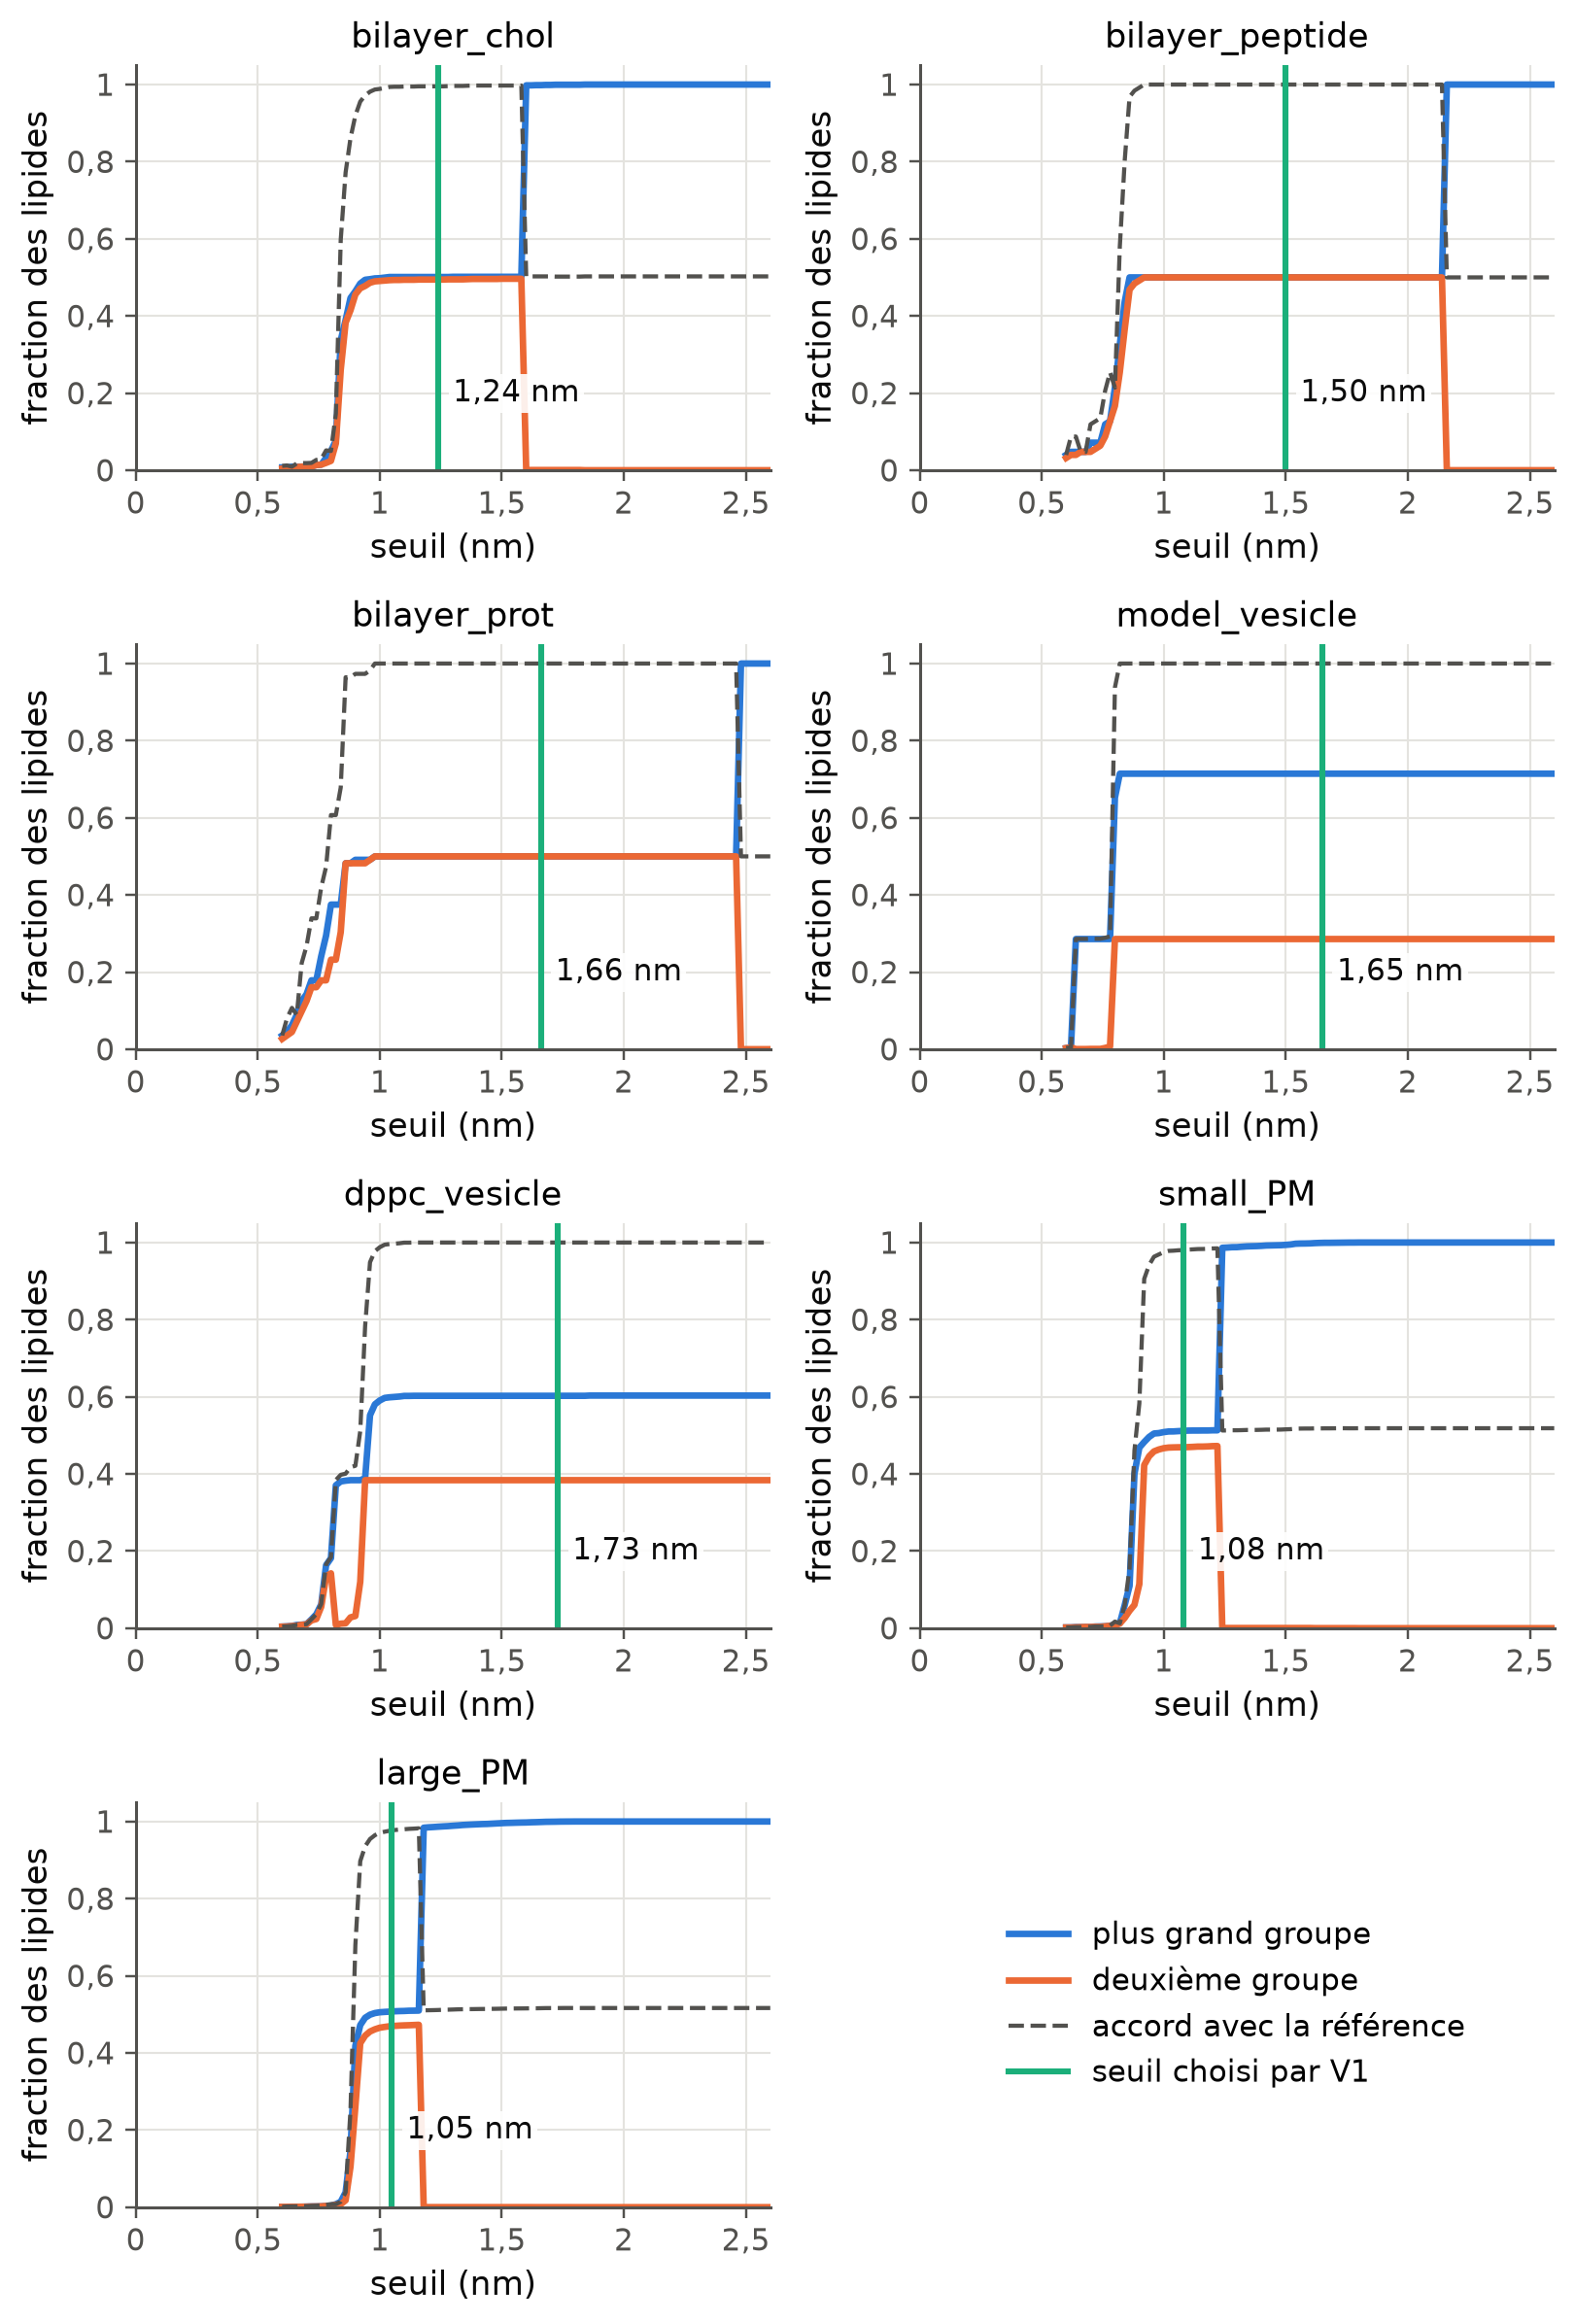
\includegraphics[width=0.82\textwidth]{../resultats/figures/fig_balayage_seuil.png}
\caption{Taille des deux plus grands groupes selon le seuil. Bleu~: plus grand groupe~; orange~: deuxième~;
tirets~: taux de bonnes réponses~; vert~: seuil choisi automatiquement par V1. La « bonne » plage est celle où
bleu et orange forment chacun un plateau. Elle est large pour les membranes simples, mais très étroite (environ
0,25\,nm) pour les membranes plasmiques.}
\end{figure}

\subsection{Résultat}
De 99,7 à 100\,\% de lipides bien placés. La figure montre la faiblesse de la méthode~: sur les membranes
plasmiques, la plage du bon seuil est très étroite. Un seuil fixé « au hasard » échouerait complètement, et la
réussite dépend du choix, fait à la main, de l'atome de tête de chaque type de lipide.

\fichiers{%
\f{src/leaflet.cpp}, fonction \f{graph\_auto}~: l'algorithme de la V1.\\
\f{resultats/figures/fig\_balayage\_seuil.png}~: la figure ci-dessus.\\
\f{resultats/structures/balayage\_seuil.csv}~: les données de cette figure.\\
\f{resultats/structures/<membrane>/V1\_leaflets.txt}~: les feuillets trouvés par V1 pour chaque membrane.}

%=====================================================================
\section{Point 2 -- Sans atome de référence défini à l'avance (V2)}
%=====================================================================
\subsection{Le problème}
En V1, il faut indiquer à la main le nom de l'atome de tête de chaque type de lipide. Avec 63 types de lipides,
c'est long et source d'erreurs. Le point~2 demande que le programme le trouve tout seul.

\subsection{L'idée : utiliser la chimie des lipides}
\begin{itemize}
\item Un atome situé \textbf{au cœur} de la membrane est entouré d'autres lipides \textbf{de tous les côtés}.
\item Un atome de la \textbf{tête}, à la surface, n'a de voisins lipidiques \textbf{que d'un côté}, l'autre côté
étant l'eau.
\end{itemize}
Pour chaque atome, le programme calcule la position moyenne de ses voisins lipidiques (dans un rayon de 1\,nm). Si
les voisins sont répartis tout autour, cette moyenne tombe sur l'atome lui-même~; s'ils sont d'un seul côté, elle
s'en écarte. Cet écart s'appelle l'\textbf{exposition}. Pour chaque type de lipide, l'atome le plus exposé
devient automatiquement « la tête ».

Pour les lipides dont la tête est petite et peu exposée (cholestérol, diacylglycérols, céramides), une deuxième
règle est appliquée~: on choisit l'atome le plus proche des têtes des lipides voisins.

Ce calcul n'est fait \textbf{qu'une seule fois}, sur la première image~; il prend de 8 à 162\,ms. Ensuite, la V2
fonctionne exactement comme la V1.

\subsection{Résultat}
Les têtes trouvées sont cohérentes avec la chimie (par exemple \f{NC3} pour les phosphatidylcholines, \f{NH3}
pour les phosphatidyléthanolamines, \f{ROH} pour le cholestérol). Les performances sont les mêmes qu'en V1, mais
\textbf{sans aucune information donnée à la main}.

\fichiers{%
\f{src/leaflet.cpp}, fonction \f{detect\_heads}~: la détection automatique.\\
\f{resultats/structures/tetes\_detectees.txt}~: pour chaque type de lipide, la tête « officielle » et la tête
trouvée automatiquement.\\
\f{resultats/structures/<membrane>/V2\_leaflets.txt}~: les feuillets trouvés par V2.\\
Commande pour afficher les têtes détectées~: \f{./bin/leaflet -f <fichier.gro> --heads -m 2}}

%=====================================================================
\section{Point 3 -- Orientation et normale locale (V3)}
%=====================================================================
\subsection{Deux notions}
\begin{itemize}
\item \textbf{L'orientation d'un lipide}~: la flèche qui va du centre de la molécule vers sa tête. Elle pointe
toujours vers l'eau, donc vers le haut dans le feuillet du haut et vers le bas dans le feuillet du bas.
\item \textbf{La normale locale}~: la direction perpendiculaire à la surface de la membrane, autour d'un lipide.
Sur une vésicule, elle change d'un endroit à l'autre (elle pointe vers l'extérieur de la bulle).
\end{itemize}

\subsection{Le calcul de la normale}
Pour chaque lipide, on prend les têtes des voisins situés à moins de 2\,nm et orientés dans le même sens que lui.
Ces têtes forment localement une sorte de « disque » de points. La normale est la direction dans laquelle ce
disque est le \textbf{moins épais}. Mathématiquement, c'est une \emph{analyse en composantes principales}~: on
calcule une matrice $3\times3$ et on cherche sa plus petite valeur propre. C'est la même technique que celle
utilisée pour reconstruire des surfaces à partir de nuages de points (Lidar), comme le suggère l'énoncé.

\subsection{La règle pour relier deux lipides}
Deux lipides proches (moins de 1,5\,nm) ne sont reliés que si \textbf{leurs normales pointent dans le même sens}.
Deux lipides de feuillets différents ont des normales opposées~: ils ne sont donc \textbf{jamais reliés}, même
avec un seuil de distance généreux. Résultat~: \textbf{on n'a plus besoin de chercher le seuil}, une valeur fixe
suffit.

\subsection{Résultat}
Une méthode robuste (99,75 à 100\,\%), mais c'est \textbf{la plus lente} des versions, à cause du calcul de normale
pour chaque lipide.

\fichiers{%
\f{src/leaflet.cpp}, fonction \f{graph\_oriented} (partie \f{ver == 3}) et fonction \f{smallest\_eigvec}
(calcul de la normale).\\
\f{resultats/structures/<membrane>/V3\_leaflets.txt}~: les feuillets trouvés par V3.}

%=====================================================================
\section{Point 4 -- La version finale (V4) et sa justification}
%=====================================================================
\subsection{Ce qu'on a appris des versions 1 à 3}
\begin{itemize}
\item C'est \textbf{l'orientation} qui sépare vraiment les feuillets. Le seuil automatique de V1/V2 n'est qu'un
moyen détourné d'y arriver.
\item Le calcul de normale par analyse en composantes principales (V3) est \textbf{coûteux} et n'apporte pas plus
de précision.
\item Les cas difficiles sont des lipides \textbf{isolés au milieu} de la membrane (surtout le cholestérol).
\end{itemize}

\subsection{La version finale garde seulement l'essentiel}
\begin{enumerate}
\item la tête est détectée automatiquement (comme en V2)~;
\item on calcule l'orientation de chaque lipide~;
\item on cherche les voisins une seule fois, à 1,5\,nm~;
\item la normale est simplement la \textbf{moyenne des orientations des voisins}, beaucoup moins chère que
l'analyse en composantes principales~;
\item on ne relie que des lipides proches, bien orientés, et dont le voisinage est clairement d'un seul
feuillet~; les lipides à petite tête enfouie (cholestérol, diacylglycérols, céramides) ne servent pas à
construire les feuillets~;
\item les lipides ambigus (par exemple un cholestérol couché au milieu) sont rattachés ensuite au feuillet de
leur plus proche voisin.
\end{enumerate}

\subsection{Justification (ce que demande l'énoncé)}
\begin{itemize}
\item \textbf{Fiabilité}~: même précision que les autres versions (99,77 à 100\,\%).
\item \textbf{Temps de calcul}~: 1,6 à 2,8 fois plus rapide que V1, V2 et V3.
\item \textbf{Robustesse}~: aucun réglage à faire selon la membrane~; l'orientation empêche les deux feuillets de
fusionner même si les distances sont trompeuses.
\end{itemize}

\subsection{Une correction apportée grâce à la trajectoire}
Sur la trajectoire de la surfactine, la première version de V4 fusionnait les deux feuillets sur 30 images sur 1001.
En cherchant les liens fautifs, on a trouvé une dizaine de cholestérols couchés au milieu de la membrane, qui
reliaient les deux feuillets. Leur petite tête (\f{ROH}) est enfouie et ils ont des voisins des deux côtés. La
correction~: ces lipides ne servent plus à \emph{construire} les feuillets, ils y sont seulement \emph{rattachés}
ensuite. Résultat~: plus aucune image fusionnée, et la même précision qu'avant sur les 7 structures.

\subsection{La V5, pour vérifier}
La V5 est la V4 sans l'étape 4 (sans moyenne des orientations). C'est une \textbf{ablation}~: on retire un
élément pour voir s'il sert à quelque chose. La V5 donne presque les mêmes résultats~; on garde quand même la
moyenne en V4, car elle coûte peu et rend la méthode moins sensible aux lipides très inclinés.

\subsection{Les rares erreurs}
Toutes les erreurs restantes sont des molécules de \textbf{cholestérol} (et 2 diacylglycérols) dont la tête est
à moins de 0,8\,nm du milieu de la membrane. Ce sont des molécules en train de passer d'un feuillet à l'autre~:
leur feuillet est réellement ambigu.

\begin{figure}[H]\centering
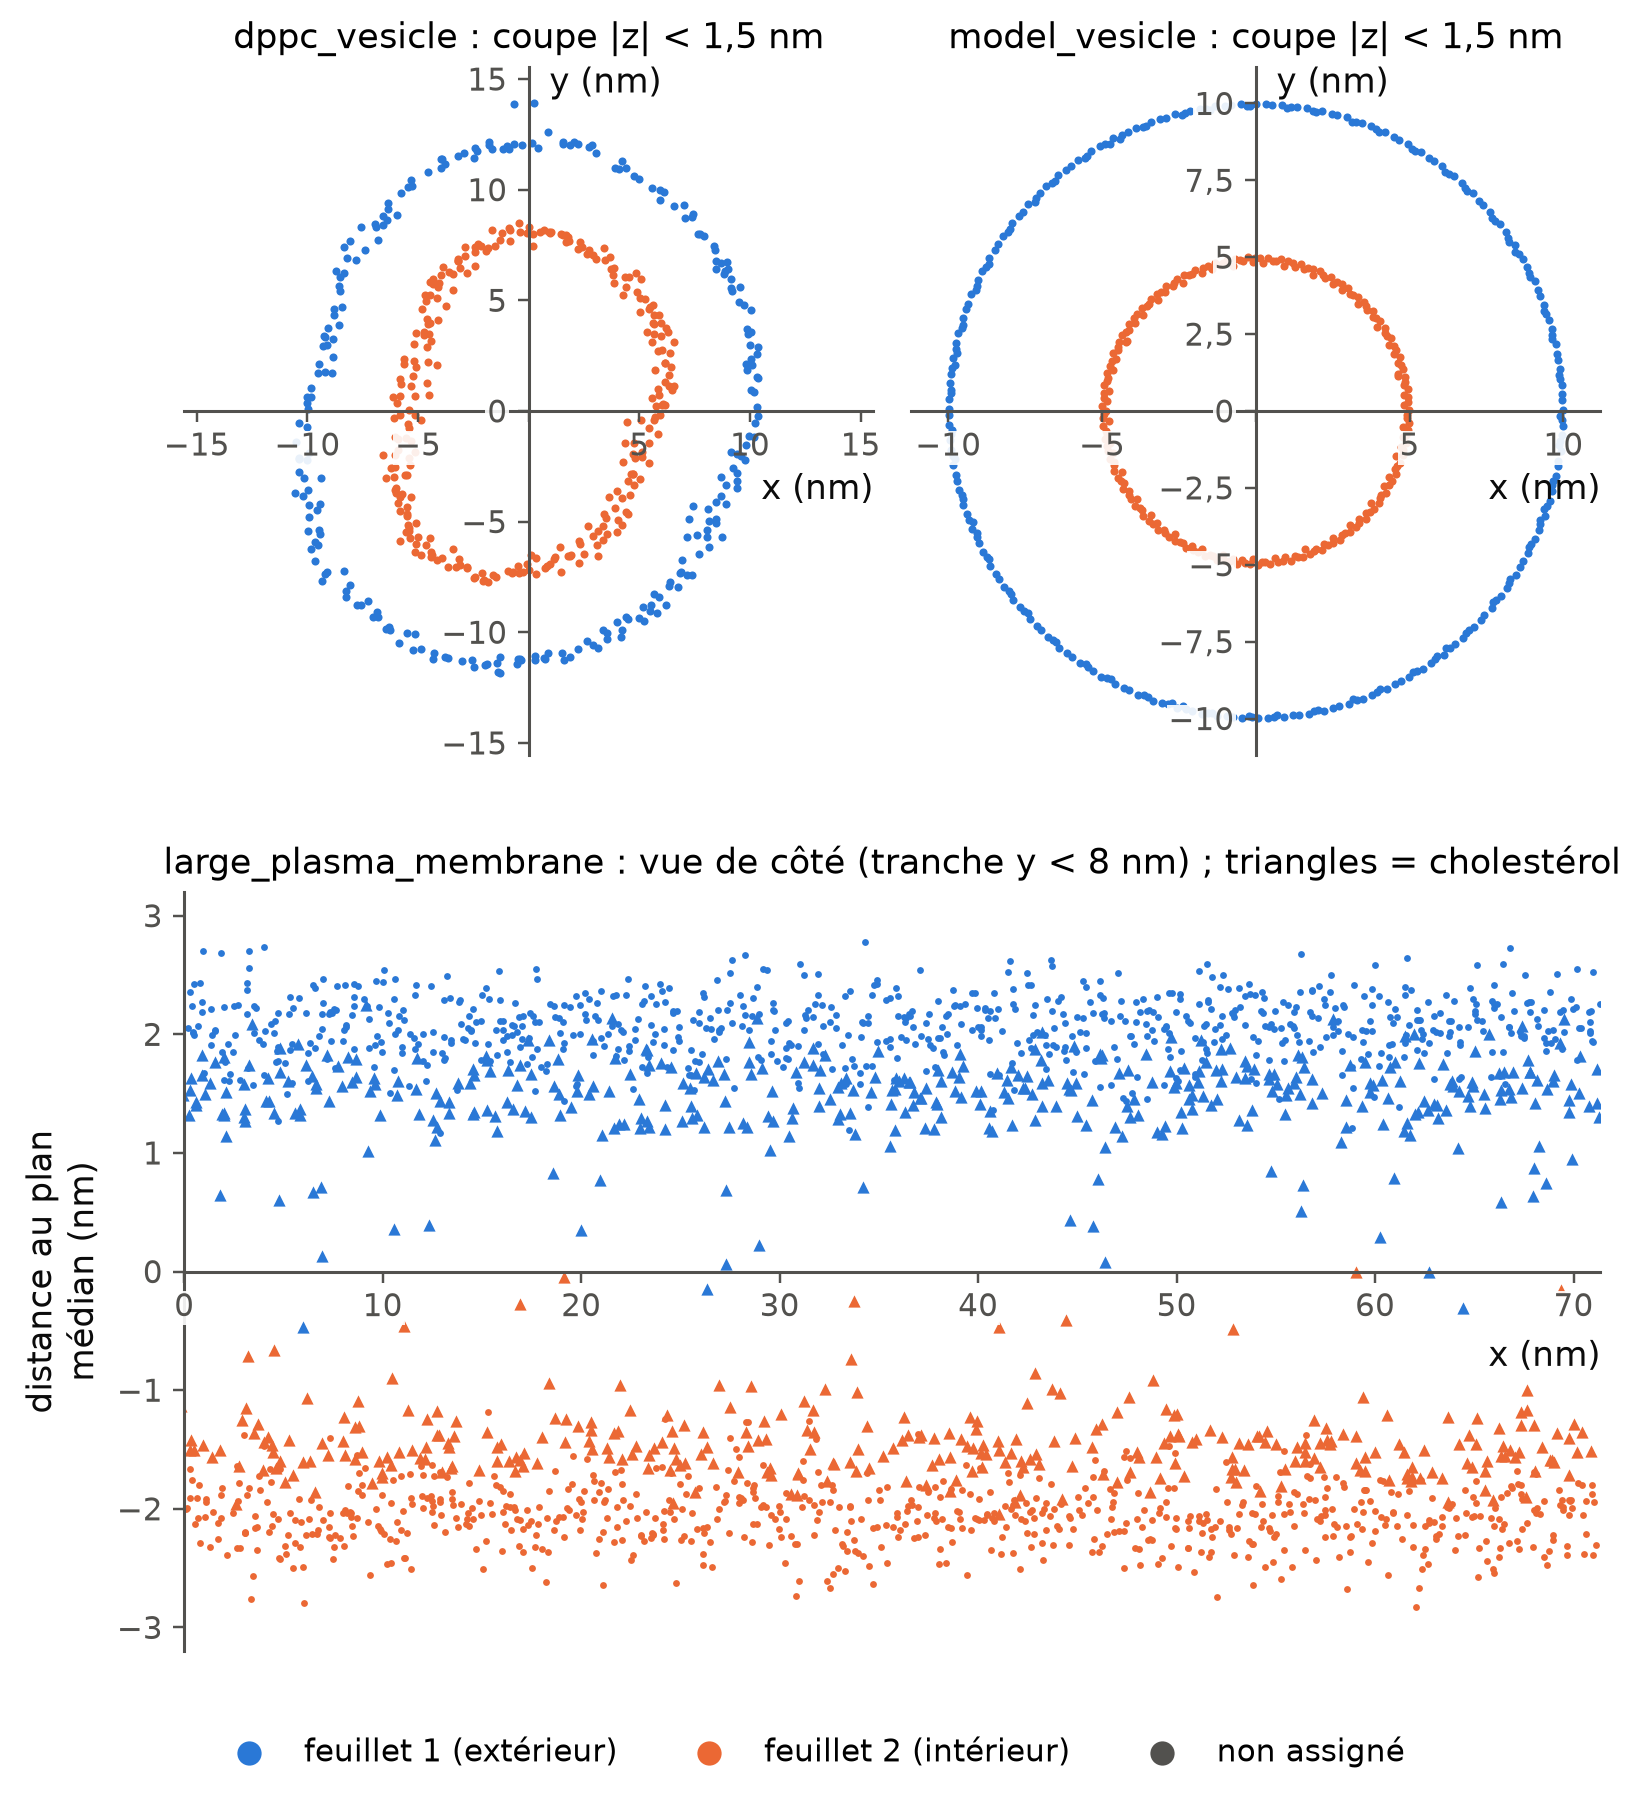
\includegraphics[width=0.92\textwidth]{../resultats/figures/fig_feuillets.png}
\caption{Les feuillets trouvés par V4, en deux couleurs. À gauche et au centre, les deux vésicules coupées en
deux~: on voit bien le feuillet extérieur (bleu) et le feuillet intérieur (orange). À droite, la grande membrane
vue de côté~: les points isolés au milieu sont des cholestérols.}
\end{figure}

\fichiers{%
\f{src/leaflet.cpp}~: version utilisée par défaut (\f{-m 4})~; la V5 correspond à \f{-m 5}.\\
\f{resultats/structures/<membrane>/V4\_leaflets.txt} et \f{V5\_leaflets.txt}~: les feuillets trouvés.\\
\f{resultats/figures/fig\_feuillets.png}~: la figure ci-dessus.\\
\f{resultats/structures/analyse\_erreurs.txt}~: la liste et la nature des erreurs de V4.}

%=====================================================================
\section{Point 5 -- Application à une trajectoire}
%=====================================================================
\subsection{Ce qui est fait}
\begin{enumerate}
\item On lit la trajectoire image par image.
\item La tête de chaque type de lipide est détectée une seule fois, sur la première image.
\item La V4 est appliquée à chaque image, et on chronomètre le calcul.
\item On compare les feuillets d'une image à l'autre, pour repérer les lipides qui changent de feuillet.
\item Pour mesurer la vitesse « en continu », on refait l'analyse sur environ 2000 images (les 1001 images de
\f{prod1.xtc} deux fois), d'abord sur un seul cœur, puis en répartissant les images sur les 12 threads.
\item On compare avec V1, FATSLiM et LeafletFinder sur les mêmes images (point~6).
\end{enumerate}

\subsection{Les difficultés propres à cette trajectoire}
\begin{itemize}
\item \textbf{Des molécules sur plusieurs résidus.} Dans les 7 structures, un lipide = un résidu. Ici, un
glucosylcéramide est écrit sur deux résidus (le sucre et le céramide) et une surfactine sur huit. Le programme lit
donc le découpage exact en molécules dans \f{prod.tpr}. Sans cela, il trouvait 3744 «~lipides~» au lieu de 3040.
\item \textbf{La surfactine n'est pas un lipide de la membrane}~: elle est exclue de l'analyse (option
\f{--exclude S14}).
\item \textbf{Pas de bonne réponse fournie.} Il n'y a pas de \f{leaflets.txt} pour la trajectoire. On juge donc la
fiabilité de trois façons~: l'accord avec FATSLiM et V1~; une référence géométrique (la tête est-elle au-dessus ou
au-dessous du milieu local de la membrane~?)~; et la logique physique (les phospholipides ne doivent presque jamais
changer de feuillet, le cholestérol si).
\end{itemize}

\subsection{Résultats}
\begin{itemize}
\item \textbf{Temps}~: 1,3\,ms par image (3040 lipides, 83\,095 particules). Les 1001 images de \f{prod1.xtc} sont
analysées en 1,3\,s, contre 28,7\,s pour FATSLiM et 87\,s pour LeafletFinder. En répartissant les images sur les
12 threads, on traiterait 100\,000 images en environ 28 secondes.
\item \textbf{Fiabilité}~: V4 est d'accord avec FATSLiM à 99,75\,\% et avec V1 à 99,85\,\%. Aucune image n'est
fusionnée. LeafletFinder, avec son seuil par défaut, fusionne les feuillets sur 96\,\% des images.
\item \textbf{Physique}~: sur les 20\,µs de production, environ 300 lipides changent de feuillet par µs, et ce sont
\textbf{tous des cholestérols}~; aucun phospholipide ni glycolipide ne change de feuillet. C'est exactement ce qu'on
attend.
\item \textbf{Limite}~: quand les images sont très rapprochées (5\,ps), environ 5 cholestérols ambigus changent
d'assignation d'une image à l'autre. Ce n'est pas un vrai basculement~; toutes les méthodes le font (FATSLiM un
peu plus).
\end{itemize}

\textbf{Remarque}~: les temps ont été mesurés sur batterie, avec d'autres applications ouvertes. Pour des mesures
plus nettes, lancer \f{resultats/relance\_tout.sh} sur secteur~; tableaux et figures se mettent à jour.

\fichiers{%
\f{Surfactine-R1/}~: la trajectoire du cours.\\
\f{scripts/run\_trajectory.py}~: le script du point~5 (il fait aussi la comparaison du point~6 sur la
trajectoire).\\
\f{scripts/xtc\_to\_gro.py}~: convertit un \f{.xtc} en \f{.gro} à plusieurs images, pour que \f{bin/leaflet}
traite la trajectoire seul.\\
\f{scripts/tpr\_molsizes.py}~: extrait le découpage en molécules du \f{.tpr} pour \f{bin/leaflet}.\\
\f{scripts/analyse\_types\_trajectoire.py}~: quels types de lipides changent de feuillet.\\
\f{resultats/trajectoire\_surfactine\_prod1/}~: les 1001 images de \f{prod1.xtc}.\\
\f{resultats/trajectoire\_surfactine\_20us/}~: la production de 20\,µs.\\
\f{resultats/trajectoire\_surfactine\_prodtrr/}~: les 61 images lisibles de \f{prod.trr}.\\
\f{resultats/trajectoire/}~: la trajectoire de test DPPC.\\
Dans chacun~: \f{resume.txt} (bilan lisible), \f{par\_trame.csv} (détail image par image),
\f{feuillets\_V4.txt} (feuillets de chaque image).\\
\f{resultats/figures/fig\_trajectoire\_temps.png}, \f{fig\_surfactine\_20us.png},
\f{fig\_surfactine\_vue.png}~: les figures.\\
\f{resultats/relance\_tout.sh}~: relance tous les calculs.}

%=====================================================================
\section{Point 6 -- Comparaison avec LeafletFinder et FATSLiM}
%=====================================================================
\subsection{Les deux outils existants}
\begin{itemize}
\item \textbf{LeafletFinder} (bibliothèque Python MDAnalysis)~: un graphe avec un seuil, comme notre V1. Testé
avec son seuil par défaut (15\,Å, soit 1,5\,nm) puis avec un seuil optimisé par sa fonction
\f{optimize\_cutoff}.
\item \textbf{FATSLiM}~: un outil fondé sur les normales locales, comme notre V3.
\end{itemize}

\subsection{Comment on compare}
Chaque méthode est lancée sur les 7 membranes et sur la trajectoire. On mesure~:
\begin{itemize}
\item le \textbf{pourcentage de lipides bien placés}, par rapport aux fichiers \f{leaflets.txt}~;
\item le \textbf{temps de calcul}, sur un seul thread pour que la comparaison soit équitable, et aussi sur
12 threads.
\end{itemize}

\subsection{Résultats principaux}
\begin{table}[H]\centering\small
\begin{tabular}{|l|l|l|}\hline
Méthode & Fiabilité & Temps (grande membrane, 1 thread)\\\hline
V4 (finale) & 99,77 à 100\,\% & \textbf{7,5\,ms}\\\hline
FATSLiM & 99,82 à 100\,\% & 210\,ms\\\hline
LeafletFinder 15\,Å & 51\,\% sur les membranes plasmiques (échec) & 1400\,ms\\\hline
LeafletFinder optimisé & 98,2 à 98,5\,\% sur les membranes plasmiques & 42\,000\,ms\\\hline
\end{tabular}
\caption{Résumé de la comparaison (détails dans le rapport, tableaux 3 à 5).}
\end{table}
\begin{itemize}
\item \textbf{V4} est aussi fiable que FATSLiM, mais \textbf{28 à 250 fois plus rapide}.
\item \textbf{LeafletFinder} échoue sur les membranes plasmiques avec son seuil par défaut~: tous les lipides
fusionnent en un seul groupe. Avec un seuil optimisé, il atteint 98\,\%, mais met jusqu'à 39 secondes.
\item \textbf{FATSLiM} retrouve presque toujours exactement la bonne réponse~: les fichiers \f{leaflets.txt} ont
très probablement été produits avec lui.
\end{itemize}

\begin{figure}[H]\centering
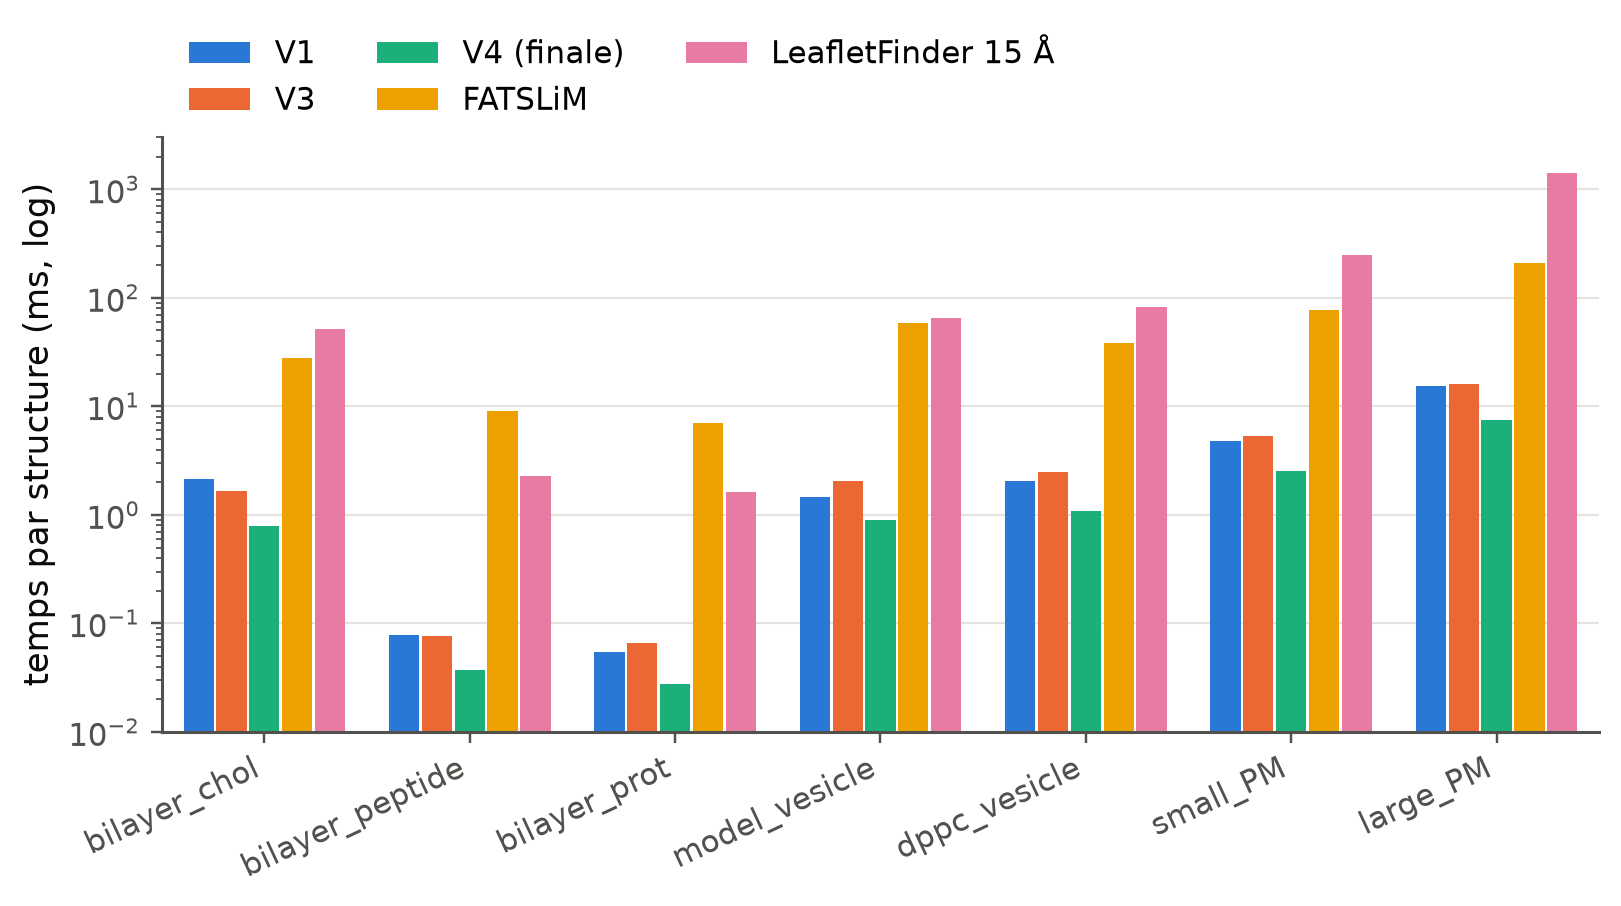
\includegraphics[width=0.95\textwidth]{../resultats/figures/fig_temps_structures.png}
\caption{Temps de calcul pour chaque membrane (échelle logarithmique~: chaque graduation multiplie par 10).
La V4 (en vert) est toujours la plus rapide.}
\end{figure}

\fichiers{%
\f{scripts/benchmark\_structures.py}~: le script de comparaison sur les 7 membranes.\\
\f{resultats/structures/resultats.csv}~: le tableau complet (une ligne par membrane et par méthode).\\
\f{resultats/structures/<membrane>/LeafletFinder\_*.txt}, \f{FATSLiM\_leaflets.txt}~: leurs résultats.\\
\f{resultats/structures/scalabilite\_threads.csv} et \f{resultats/figures/fig\_threads.png}~: le gain selon le
nombre de threads.\\
\f{resultats/figures/fig\_temps\_structures.png}~: la figure ci-dessus.\\
\f{resultats/benchmark\_log.txt}~: le journal complet de l'exécution.}

%=====================================================================
\section{Vérifier soi-même que les résultats sont justes}
%=====================================================================
\subsection{Le principe}
Pour les 7 structures, on dispose de la bonne réponse (\f{leaflets.txt}). Le script
\f{scripts/verifier\_resultats.py} compare, \textbf{lipide par lipide}, ce que chaque méthode a trouvé avec cette
bonne réponse. Pour chaque lipide, il y a quatre cas possibles~:
\begin{itemize}
\item \textbf{correct}~: dans le bon feuillet~;
\item \textbf{mauvais feuillet}~: dans l'autre feuillet~;
\item \textbf{non assigné}~: la méthode n'a pas su le placer~;
\item \textbf{groupe parasite}~: la méthode l'a mis dans un petit groupe en plus des deux feuillets (cas fréquent
avec LeafletFinder).
\end{itemize}
Le script vérifie aussi que les fichiers de résultats enregistrés sont identiques à un calcul refait au moment de la
vérification.

\subsection{Ce qu'on obtient}
\begin{itemize}
\item V4 place correctement \textbf{tous} les lipides de 5 membranes sur 7.
\item Il reste 3 erreurs sur 1944 (\f{bilayer\_chol}), 14 sur 6664 (petite membrane plasmique) et 44 sur 19\,239
(grande membrane plasmique). \textbf{Ce sont presque toutes des cholestérols} (plus 2 diacylglycérols), placés près
du milieu de la membrane~: des molécules en train de changer de feuillet, dont la place est réellement ambiguë.
\item Sur la trajectoire du cours, il n'y a pas de bonne réponse~: on compare V4 à FATSLiM, à V1 et à la position de
la tête (au-dessus ou au-dessous du milieu local de la membrane). V4 diffère de chacun pour 2 à 8 lipides sur 3040,
\textbf{uniquement des cholestérols} situés à environ 0,1\,nm du milieu de la membrane.
\end{itemize}

\begin{figure}[H]\centering
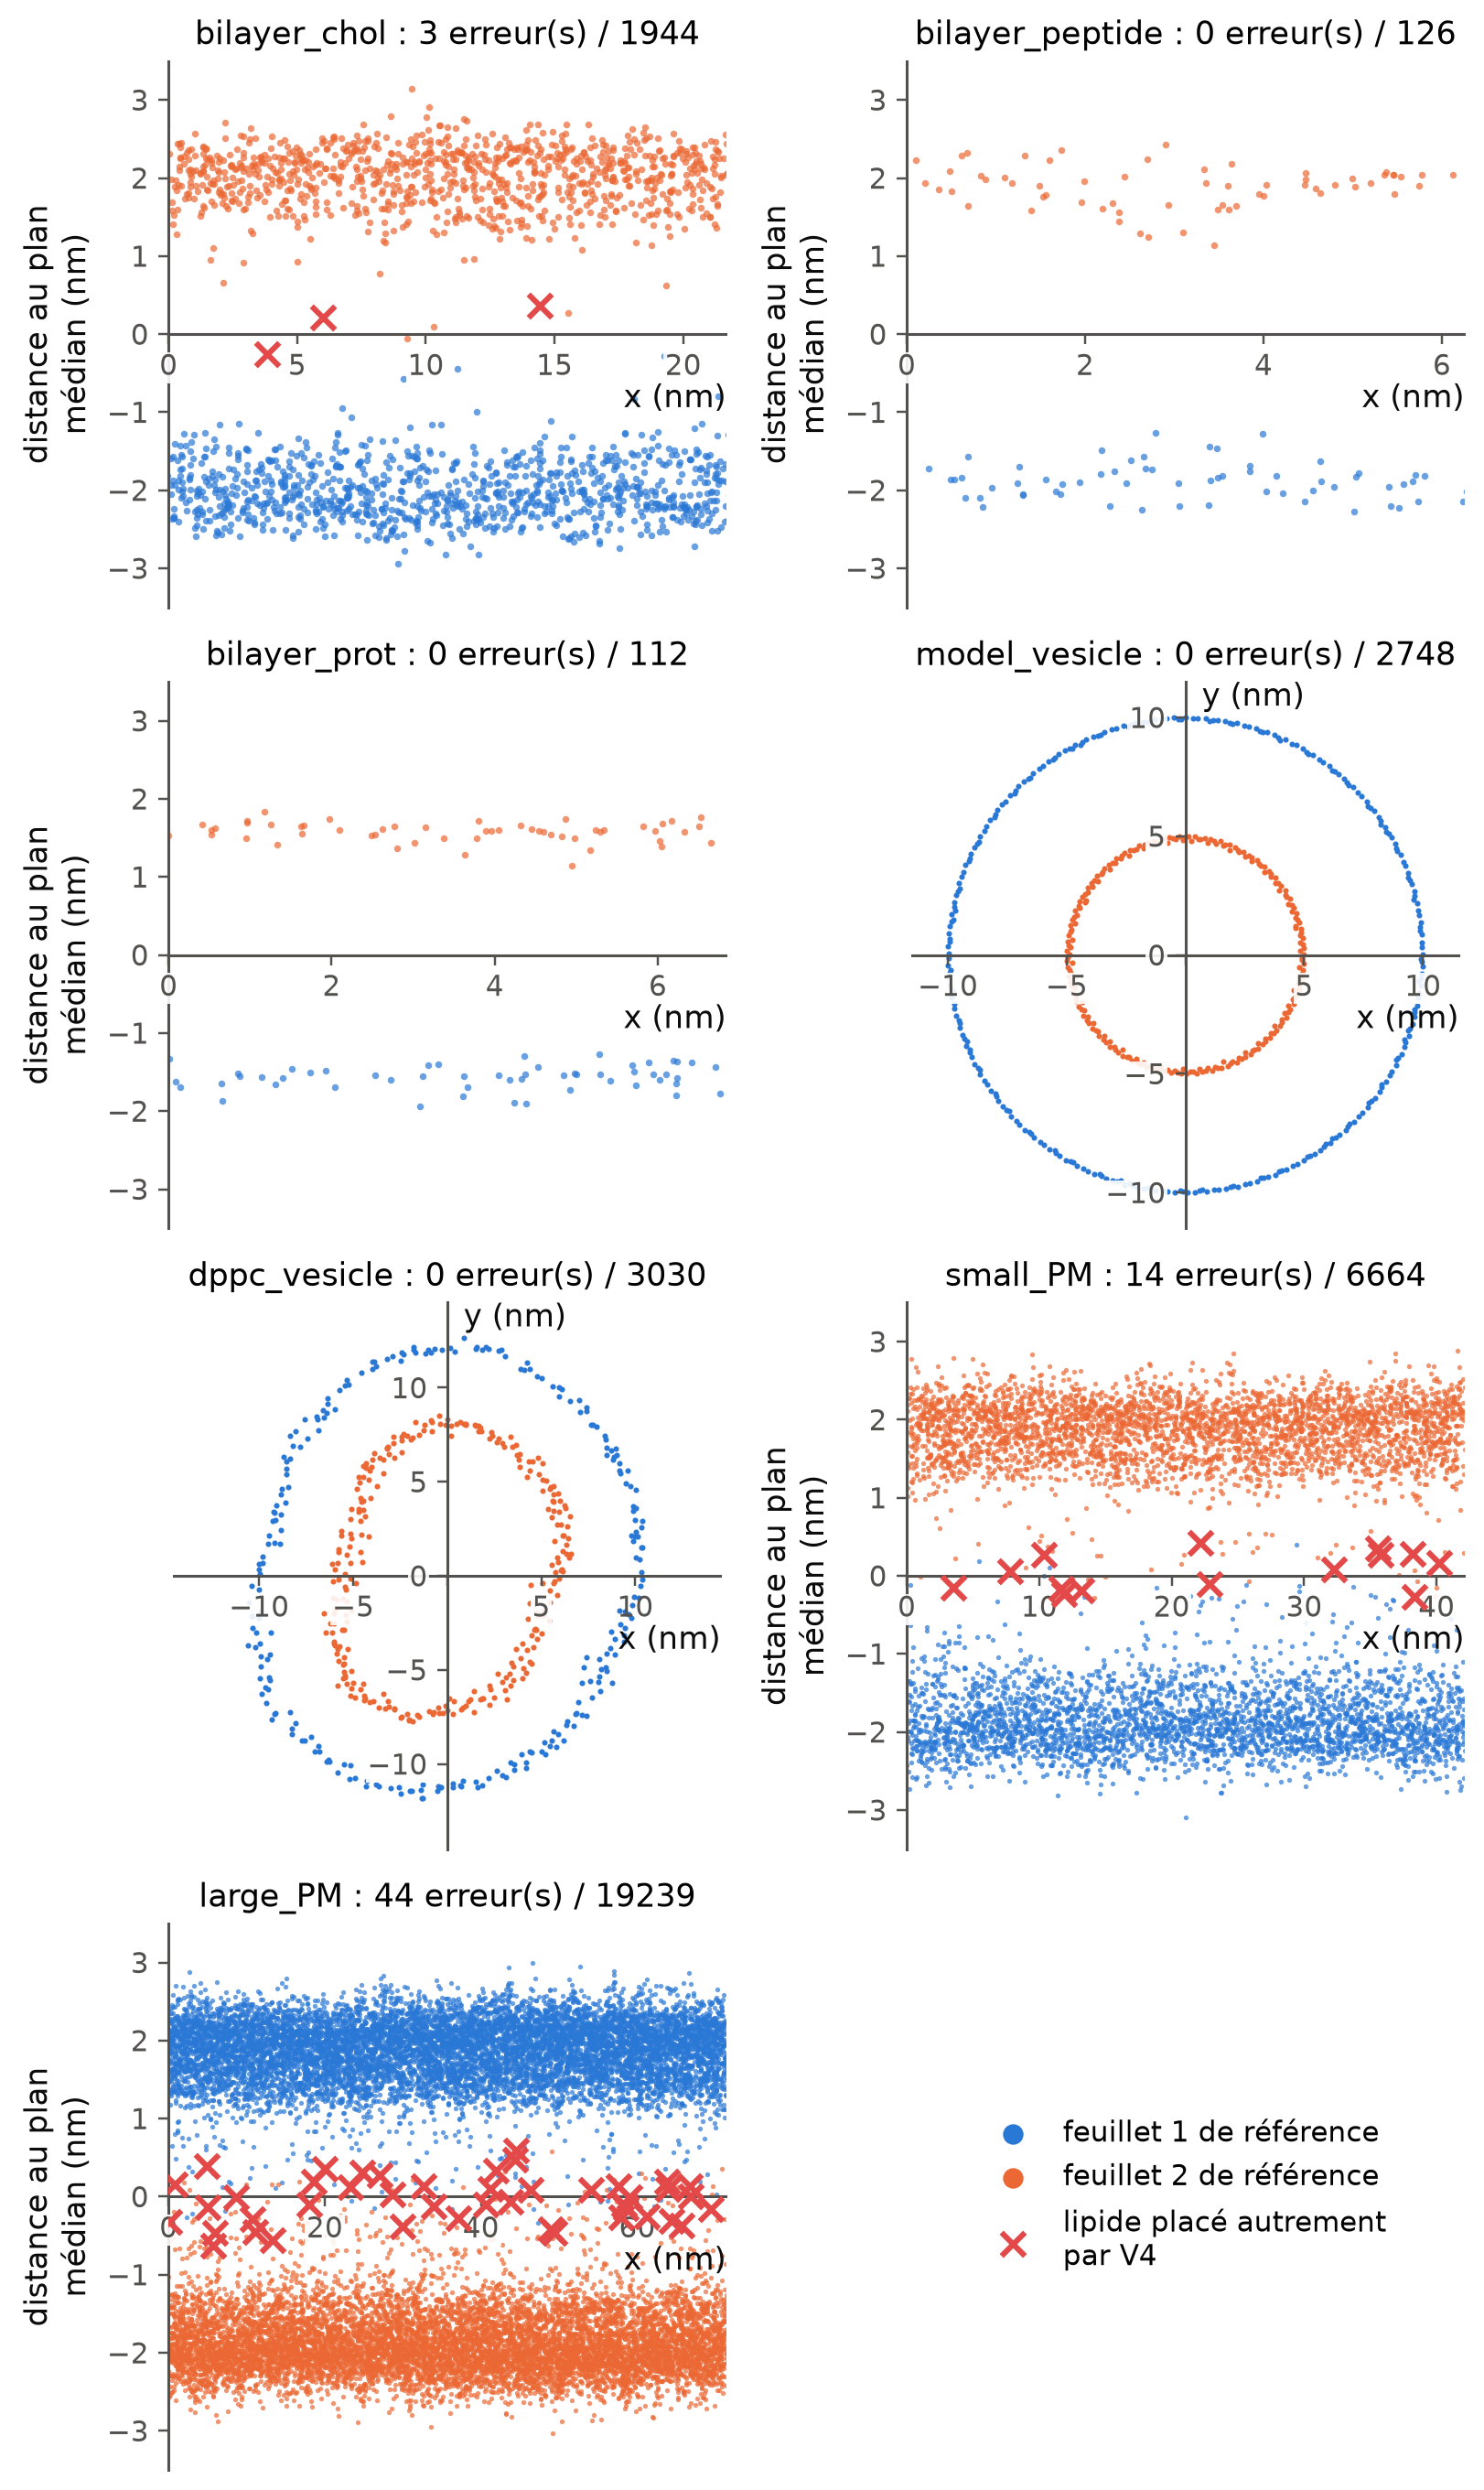
\includegraphics[width=0.70\textwidth]{../resultats/verification/fig_verification.png}
\caption{En bleu et orange, les deux feuillets de la bonne réponse~; en croix rouges, les lipides que V4 place
autrement. Toutes les croix sont près de la ligne en tirets, le milieu de la membrane.}
\end{figure}

\fichiers{%
\f{resultats/verification/resume\_verification.txt}~: \textbf{le tableau à lire en premier}~: pour chaque membrane et
chaque méthode, le nombre de lipides corrects, mal placés, non assignés, et les types de lipides en erreur.\\
\f{resultats/verification/<membrane>\_V4\_lipides.csv}~: une ligne \emph{par lipide}~: son numéro, son type, le
feuillet attendu, le feuillet trouvé par V4, sa position et son orientation. S'ouvre avec LibreOffice.\\
\f{resultats/verification/<membrane>\_<méthode>\_erreurs.csv}~: uniquement les lipides mal placés, pour chaque méthode.\\
\f{resultats/verification/trajectoire\_surfactine\_trame00\_lipides.csv} et \f{trame20}~: la même chose pour la
trajectoire du cours (V4, FATSLiM, V1 et la position de la tête, lipide par lipide).\\
\f{resultats/verification/vmd\_<membrane>.tcl}~: pour \emph{voir} les erreurs dans VMD (les lipides mal placés en
rouge, les feuillets attendus en bleu et orange).\\
\f{resultats/verification/fig\_verification.png}~: la figure ci-dessus.}

\subsection{Les commandes}
Depuis le dossier du projet (\f{cd \textasciitilde/Documents/"projet membranne lipidique"})~:
\begin{lstlisting}
# 1. Tout relancer d'un coup (compilation, calculs, vérification, figures, PDF) ~ 15 min
bash resultats/relance_tout.sh

# 2. Ou seulement la vérification (1 min), une fois les calculs faits
.venv/bin/python scripts/verifier_resultats.py
less resultats/verification/resume_verification.txt

# 3. Voir les erreurs d'une membrane dans VMD
vmd -e resultats/verification/vmd_large_plasma_membrane.tcl

# 4. Vérifier une membrane à la main avec le programme C++ seul
./bin/leaflet -f Projet3/bilayer_chol/bilayer_chol.gro -m 4 \
              -r Projet3/bilayer_chol/leaflets.txt -o mes_feuillets.txt
\end{lstlisting}
La commande 4 affiche directement le pourcentage d'accord avec la bonne réponse et écrit les feuillets trouvés dans
\f{mes\_feuillets.txt}, au même format que \f{leaflets.txt}~: on peut comparer les deux fichiers.

%=====================================================================
\section{Le rapport et les fichiers annexes}
%=====================================================================
\begin{itemize}
\item \f{doc\_Projet/rapport/rapport.pdf}~: \textbf{le rapport à rendre}. Il reprend les 6 points dans l'ordre de l'énoncé.
La page de garde (noms des membres du groupe, enseignant, date) se modifie au début de \f{doc\_Projet/rapport/rapport.tex}, dans les commandes \f{\textbackslash auteurUn} à \f{\textbackslash auteurQuatre}, \f{\textbackslash enseignant} et \f{\textbackslash dateRapport}.
\item \f{doc\_Projet/rapport/tables/}~: les tableaux du rapport, générés automatiquement à partir des résultats.
\item \f{scripts/make\_figures.py} et \f{scripts/make\_tables.py}~: regénèrent les figures et les tableaux. Si l'on
relance les calculs, le rapport se met donc à jour tout seul.
\item \f{rapport/explications.pdf}~: ce document.
\item \f{README.md}~: le résumé du dossier et les commandes pour tout relancer.
\end{itemize}

\subsection{Organisation complète du dossier}
\begin{lstlisting}
projet membranne lipidique/
|-- 2026_CHPS1001_..._Lipidiques.pdf   énoncé
|-- Projet3/  Projet3.zip              les 7 membranes + bonnes réponses
|-- Surfactine-R1/                     trajectoire du cours (GROMACS, Martini 3)
|-- trajectoire/                       trajectoire de test (dppc_vesicle)
|-- src/leaflet.cpp                    TOUT le calcul (versions 1 à 5)
|-- Makefile                           compilation
|-- bin/leaflet  lib/libleaflet.so     programmes compilés
|-- scripts/
|   |-- lfpy.py                        pont Python <-> C++, calcul du taux de réussite
|   |-- benchmark_structures.py        points 1 à 4 et 6 sur les 7 membranes
|   |-- run_trajectory.py              points 5 et 6 sur une trajectoire
|   |-- xtc_to_gro.py                  conversion de trajectoire
|   |-- tpr_molsizes.py                molécules lues dans le .tpr
|   |-- analyse_types_trajectoire.py   changements de feuillet par type
|   |-- make_figures.py                figures
|   `-- make_tables.py                 tableaux du rapport
|-- resultats/
|   |-- structures/                    résultats sur les 7 membranes
|   |-- trajectoire*/                  résultats sur les trajectoires
|   |-- relance_tout.sh                relance tous les calculs
|   `-- figures/                       figures
|-- doc_Projet/
|   |-- rapport/rapport.tex  .pdf      le rapport à rendre (+ tables/)
|   `-- articles distance d'édition    sans rapport avec ce projet
|-- rapport/explications.tex  .pdf    ce document
|-- README.md
|-- .venv/  .venv-fatslim/             environnements Python (ne pas rendre)
\end{lstlisting}

\subsection{Les commandes pour tout refaire (détail des étapes)}
\begin{lstlisting}
make                                                  # compiler le C++
./bin/leaflet -f Projet3/bilayer_chol/bilayer_chol.gro -m 4 \
              -r Projet3/bilayer_chol/leaflets.txt     # tester une membrane
.venv/bin/python scripts/benchmark_structures.py       # points 1-4 et 6
.venv/bin/python scripts/run_trajectory.py             # points 5 et 6
.venv/bin/python scripts/make_figures.py               # figures
.venv/bin/python scripts/make_tables.py                # tableaux
resultats/relance_tout.sh                             # ou tout d'un coup
cd doc_Projet/rapport && pdflatex rapport.tex && pdflatex rapport.tex
\end{lstlisting}

\subsection{Ce qu'il faut rendre sur Moodle}
L'énoncé demande « un rapport ainsi que les codes et fichiers de résultats obtenus »~:
\begin{itemize}
\item le rapport~: \f{doc\_Projet/rapport/rapport.pdf}~;
\item les codes~: \f{src/}, \f{scripts/}, \f{Makefile}, \f{README.md}~;
\item les résultats~: \f{resultats/}.
\end{itemize}
Il n'est pas utile de rendre \f{.venv/}, \f{.venv-fatslim/}, \f{bin/}, \f{lib/} ni les données \f{Projet3/} et
\f{Surfactine-R1/} (842\,Mo), que l'enseignant possède déjà.

\end{document}
